\documentclass[11pt, letterpaper]{article}
\usepackage{arxiv}

\usepackage[utf8]{inputenc} % allow utf-8 input
\usepackage[T1]{fontenc}    % use 8-bit T1 fonts
\usepackage{hyperref}       % hyperlinks
\usepackage{url}            % simple URL typesetting
\usepackage{booktabs}
\usepackage{multirow}       % professional-quality tables
\usepackage{amsfonts}       % blackboard math symbols
\usepackage{nicefrac}       % compact symbols for 1/2, etc.
\usepackage{microtype}      % microtypography
\usepackage{graphicx}       % graphics
\graphicspath{{../data/results/experiments/}}
\usepackage{float}          % figure placement
\usepackage{placeins}       % FloatBarrier
\usepackage{natbib}         % citations

\title{The Impact of Text Style on Visual Focus in Vision Language Models}
\date{}
\author{
  Juan Jose Arango Serrano \\
  \texttt{s2juaran@uni-trier.de} \\
  Universität Trier\\
  \vspace{0.3cm}
  \\
  \textit{Advanced Topics in Computational Text and Media Sciences} \\
  \textit{Explainable Artificial Intelligence} \\
  Natural Language Processing \\
}

\raggedbottom
\begin{document}
\maketitle

\begin{abstract}
Vision-Language Models (VLMs) such as Qwen2-VL dynamically distribute their visual attention based on the linguistic structure and semantic tone of the text prompts they process. While standard methodologies in Explainable AI (XAI) demonstrate that these models successfully map concrete nouns to corresponding spatial coordinates, it remains unclear how minor stylistic variations, such as alternating capitalization, internet slang, or emotionally urgent tones, influence this cross modal mapping. This paper investigates whether altering the stylistic and emotional delivery of a prompt induces a structural change in the visual focus of the model, a phenomenon known as Saliency Drift. To quantify the intensity of this visual distraction, gradients were extracted directly from Layer 22 of the Qwen2-VL vision encoder, normalized into probability distributions, and evaluated using Kullback-Leibler (KL) Divergence. The findings show that structural noise, such as alternating capitalization, causes visual scattering, while abstract emotional threats (e.g., "a disaster will occur") destroy the model's ability to link words to visual features, forcing it into arbitrary spatial scanning with a KL Divergence of 0.381 from the baseline. These results show a reliability issue in current multimodal architectures. The visual attention mechanism appears influenced by linguistic noise, demonstrating that minor changes in text style can lead to significant spatial targeting errors.
\end{abstract}

\section{Introduction}
The development of Vision-Language Models (VLMs) has advanced multimodal reasoning, allowing systems to analyze visual scenes using natural language instructions \cite{bordes2024introductionvisionlanguagemodeling} and subsequent research mapped exactly how these global self-attention mechanisms replace localized convolutional features \cite{park2022visiontransformerswork}. Modern architectures such as the Qwen2-VL series \citep{wang2024qwen2vlenhancingvisionlanguagemodels} achieve visual grounding by processing images at their native resolutions and mapping specific words directly to relevant pixel regions. Within the model's transformer layers, an attention mechanism acts as a bridge, mathematically matching the words in a user's query to the corresponding visual features. This connection is what allows the model to link text to physical objects in the image.

However, an architectural vulnerability exists at the intersection of linguistic variation and cross-modal alignment. Because VLMs are trained on standard, formal datasets, their attention mechanisms develop a strong prior that correlates formal syntax with precise visual grounding. When a prompt deviates from this structure, such as through the introduction of internet slang, alternating capitalization, or an urgent tone, the query vectors of the language decoder are mathematically altered before they even interact with the visual key and value matrices \citep{bousselham2026dexardynamicexplainabilitymethod, wang2024qwen2vlenhancingvisionlanguagemodels}. This unexpected linguistic noise disrupts the cross-attention layers, causing the model to lose confidence in its visual mapping \citep{bagdasaryan2023abusing, qi2023visualadversarialexamplesjailbreak}, an effect explored in this paper as Saliency Drift.

This study examines how these simple text modifications alter the visual attention maps of the Qwen2-VL model. The results demonstrate that the visual focus of the model is very sensitive to the style of the input text, resulting in scattered attention and localization failures triggered entirely by non-visual prompt noise.

\subsection{Research Contributions}
This paper explores Multimodal Explainable AI through three key analyses. First, it applies intermediate-layer gradient extraction (specifically Layer 22) to evaluate semantic grounding. Standard explainability techniques often evaluate the final terminal layers of a network, but in vision transformers, these layers are polluted by abstract reasoning and attention sinks, leading to blurry, uninterpretable heatmaps. By extracting gradients from the middle layers, this research captures the model's visual focus precisely when cross-modal alignment is occurring.

Second, it integrates Kullback-Leibler (KL) Divergence to mathematically quantify changes in spatial attention. Since heatmaps can be subject to subjective human observation, KL Divergence provides a detailed statistical evaluation of how far a modified prompt's attention distribution has drifted from a baseline.

Finally, it highlights a specific vulnerability in cross-modal alignment: the extent to which visual processing streams are influenced by linguistic noise. The findings illustrate that minor prompt variations, such as emotional urgency or unconventional capitalization, can successfully induce spatial misalignments. This demonstrates that securing a model against adversarial visual attacks (e.g., pixel noise) is insufficient if the language channel remains an open attack vector capable of blinding the model's spatial reasoning.

\subsection{Paper Organization}
This paper is structured as follows to systematically explore and quantify the phenomenon of Saliency Drift. Section 2 provides a comprehensive review of related work, tracing the evolution of Explainable AI (XAI) from simple convolutional models to complex transformer architectures, and contextualizes recent discoveries regarding attention sinks and multimodal prompt vulnerabilities. Section 3 details the methodology. It outlines the gradient extraction process from the Qwen2-VL architecture, the mathematical formulation of Kullback-Leibler Divergence utilized for quantitative analysis, and the hardware constraints that needed 4-bit quantization and resolution downscaling. Section 4 presents the experimental design and results, dissecting the model's vulnerability to linguistic style, capitalization, emojis, and emotional urgency. Section 5 expands upon these findings through a broader discussion of safety implications and ethical considerations, before outlining current limitations and projecting future research trajectories. Finally, Section 6 concludes the paper by summarizing the findings regarding cross-modal alignment.
\section{Related Work}

\subsection{Evolution of Explainable AI in Multimodal Contexts}
The push for transparency in deep learning has led to numerous visual attribution techniques, beginning with simple Saliency Maps and Class Activation Mapping (CAM). Grad-CAM \citep{Selvaraju_2019} emerged as the standard by using the gradients of the target concept flowing into the final convolutional layer to produce a coarse localization map. However, applying such methods directly to the Transformer architectures supporting modern VLMs presents distinct challenges for explainability due to their complex multimodal nature.

Standard gradient based methods, originally built for simple image classification, often produce blurry or incorrect maps when applied to the final layers of modern architectures \citep{bousselham2026dexardynamicexplainabilitymethod}. Recent findings indicate that pulling attribution data from intermediate layers can successfully separate actual visual grounding from text based assumptions \citep{darcet2024visiontransformersneedregisters}. Thus, gradient-based methods remain very relevant, as long as they are modified to handle the specific token routing and cross-modal behaviors of vision transformers \citep{wall2026gradcamvisiontransformerssystematic}. 
.
\subsection{Attention Sinks and Prompt Vulnerabilities}
Researchers have noticed that both vision and language models sometimes dump their attention onto random, unimportant tokens. Darcet et al. \citep{darcet2024visiontransformersneedregisters} found that Vision Transformers naturally create register tokens in background image patches, which the network uses for internal math rather than looking at the image. At the same time, Xiao et al. \citep{xiao2024efficientstreaminglanguagemodels} showed that language models rely on initial attention sinks to keep their processing stable. This research connects these two ideas within Vision-Language Models. The analysis shows that when a model is overwhelmed by distracting or urgent text, it physically moves its attention away from the main subject and dumps it into these background patches, using empty visual space as an attention sink.

\subsection{Prompt Sensitivity and Model Weaknesses}

The susceptibility of VLMs to adversarial text is a growing area of concern. While early research focused mostly on visual attacks that modify pixels to fool the model \citep{qi2023visualadversarialexamplesjailbreak}, recent work has demonstrated that multimodal models are uniquely vulnerable to indirect instruction injection via text and audio \citep{bagdasaryan2023abusing}. These "jailbreaks" exploit the cross-modal alignment mechanism, using ordinary-looking text variations to overpower the visual signals. However, previous studies have largely evaluated these vulnerabilities through the lens of final text output. This paper distinguishes itself by utilizing spatial attribution to visualize exactly how and where the visual attention breaks down inside the network layers before the final text generation occurs.

Although Vision-Language Models perform very well on standard tests, their visual focus is very sensitive to changes in how a prompt is written. Recent studies point out that these models are unstable when given different natural phrasing, leading to efforts to mathematically secure their reliability \citep{yang2026semanticrobustnesscertificationvisionlanguage} and improve their general performance through training. Furthermore, recent investigations into the psychological behaviors of large language models confirm that generative systems can be very responsive to emotional stimuli, significantly altering their processing pathways when presented with urgency, stress, or threats \cite{li2023largelanguagemodelsunderstand, li2024goodbadwhyunveiling}. Additionally, research into adversarial prompts shows that emotionally charged or urgent text can successfully break the safety rules of these models \citep{zhao2023jailbreaking}. This work visually demonstrates these weaknesses, revealing that prompt sensitivity is tied to the specific image, and that extreme semantic urgency completely breaks the attention mechanism, resulting in a chaotic scattering of visual focus rather than a controlled movement to the background.

Building upon these findings, future efforts must investigate how natural conversational variations affect multimodal reliability. Unlike explicit jailbreaks that attempt to force the model into producing prohibited content \citep{zhao2023jailbreaking}, natural variations involve minor stylistic choices, such as using internet slang, omitting punctuation, or typing in all capitals. Because most large-scale pretraining datasets (such as LAION \citep{schuhmann2022laion5b}) are curated for formal grammar and clean descriptive captions, models often fail to generalize to colloquial text. When presented with these informal queries, the internal attention matrices struggle to map the unfamiliar syntactic structures to the visual embeddings \cite{yang2026semanticrobustnesscertificationvisionlanguage, yuksekgonul2023when}. Consequently, quantifying the specific impact of these stylistic choices on spatial reasoning has become a priority for the robust development of multimodal systems.

\section{Methodology}
\label{sec:methodology}

The Qwen2-VL architecture utilizes a unique mechanism for processing visual inputs. Unlike standard Vision Transformers that flatten images into 1D sequences of fixed patches, Qwen2-VL dynamically calculates a 2D macro-block grid (typically $2 \times 2$ blocks) based on the image resolution. This dynamic patching allows for flexible resolution processing but complicates standard gradient extraction. To accurately map the 1D transformer sequence back to the 2D image plane, the \texttt{get\_vision\_position\_ids} function was utilized to reconstruct the original coordinate grid.

Furthermore, gradients were explicitly extracted from the final blocks of the vision tower (specifically Layer 22) rather than the absolute final layer. As established by Darcet et al. \citep{darcet2024visiontransformersneedregisters}, the final layers of Vision Transformers frequently suffer from "attention sinks," where the model discards excess features into background patches, distorting the saliency maps. By extracting the gradients at Layer 22, the actual visual focus is recorded before it gets distorted by these sink tokens.

The resulting raw gradient magnitudes were normalized into a probability distribution $P$ where $\sum P(i) = 1$. To quantify the severity of the saliency drift between the standard baseline prompt ($P$) and the adversarial prompt ($Q$), Kullback-Leibler (KL) Divergence was employed \citep{kullback1951information}. KL Divergence is a fundamental metric in information theory that measures the statistical distance, or the amount of information lost, when one probability distribution is used to approximate another. It was specifically selected for this methodology over standard error metrics (such as Mean Squared Error) because it penalizes the model when its visual confidence drifts away from the established baseline regions. The divergence was calculated as follows:
\begin{equation}
D_{KL}(P \parallel Q) = \sum_{i} P(i) \log \left( \frac{P(i)}{Q(i)} \right)
\end{equation}
A small constant ($\epsilon = 1 \times 10^{-12}$) was added to both distributions to prevent division by zero or the logarithm of zero. This mathematical framework provides a statistical measure of visual distraction, moving beyond purely qualitative heatmap analysis. In practical terms, a KL Divergence of 0 indicates that the model's visual focus is identical to the baseline, while higher values mathematically represent the degree to which attention has scattered by the text variation.

\section{Experimental Design and Results}
This section details the qualitative and quantitative results of the prompt perturbation experiments.
\subsection{Prompt Sensitivity Based on Linguistic Style}
To determine how informal text impacts visual focus, structural text variations such as alternating capitalization (often used in internet slang) and emoji insertion were tested. As shown in Figure \ref{fig:style}, the baseline model attention (Top Left) show a low magnitude spatial distribution, with secondary activations on the foreground log and background foliage. When processing the ALL CAPS prompt, the resulting attention map displayed a massive increase in overall activation intensity. The model emitted intense attention weights across the subject, the foreground log, and scattered background patches. However, despite this intense visual scattering, the prompt produced a relatively low KL Divergence of 0.074 relative to the baseline. This indicates that while the absolute magnitude of attention increased, the relative spatial probability distribution remained structurally similar to the baseline.

\begin{figure}[H]
  \centering
  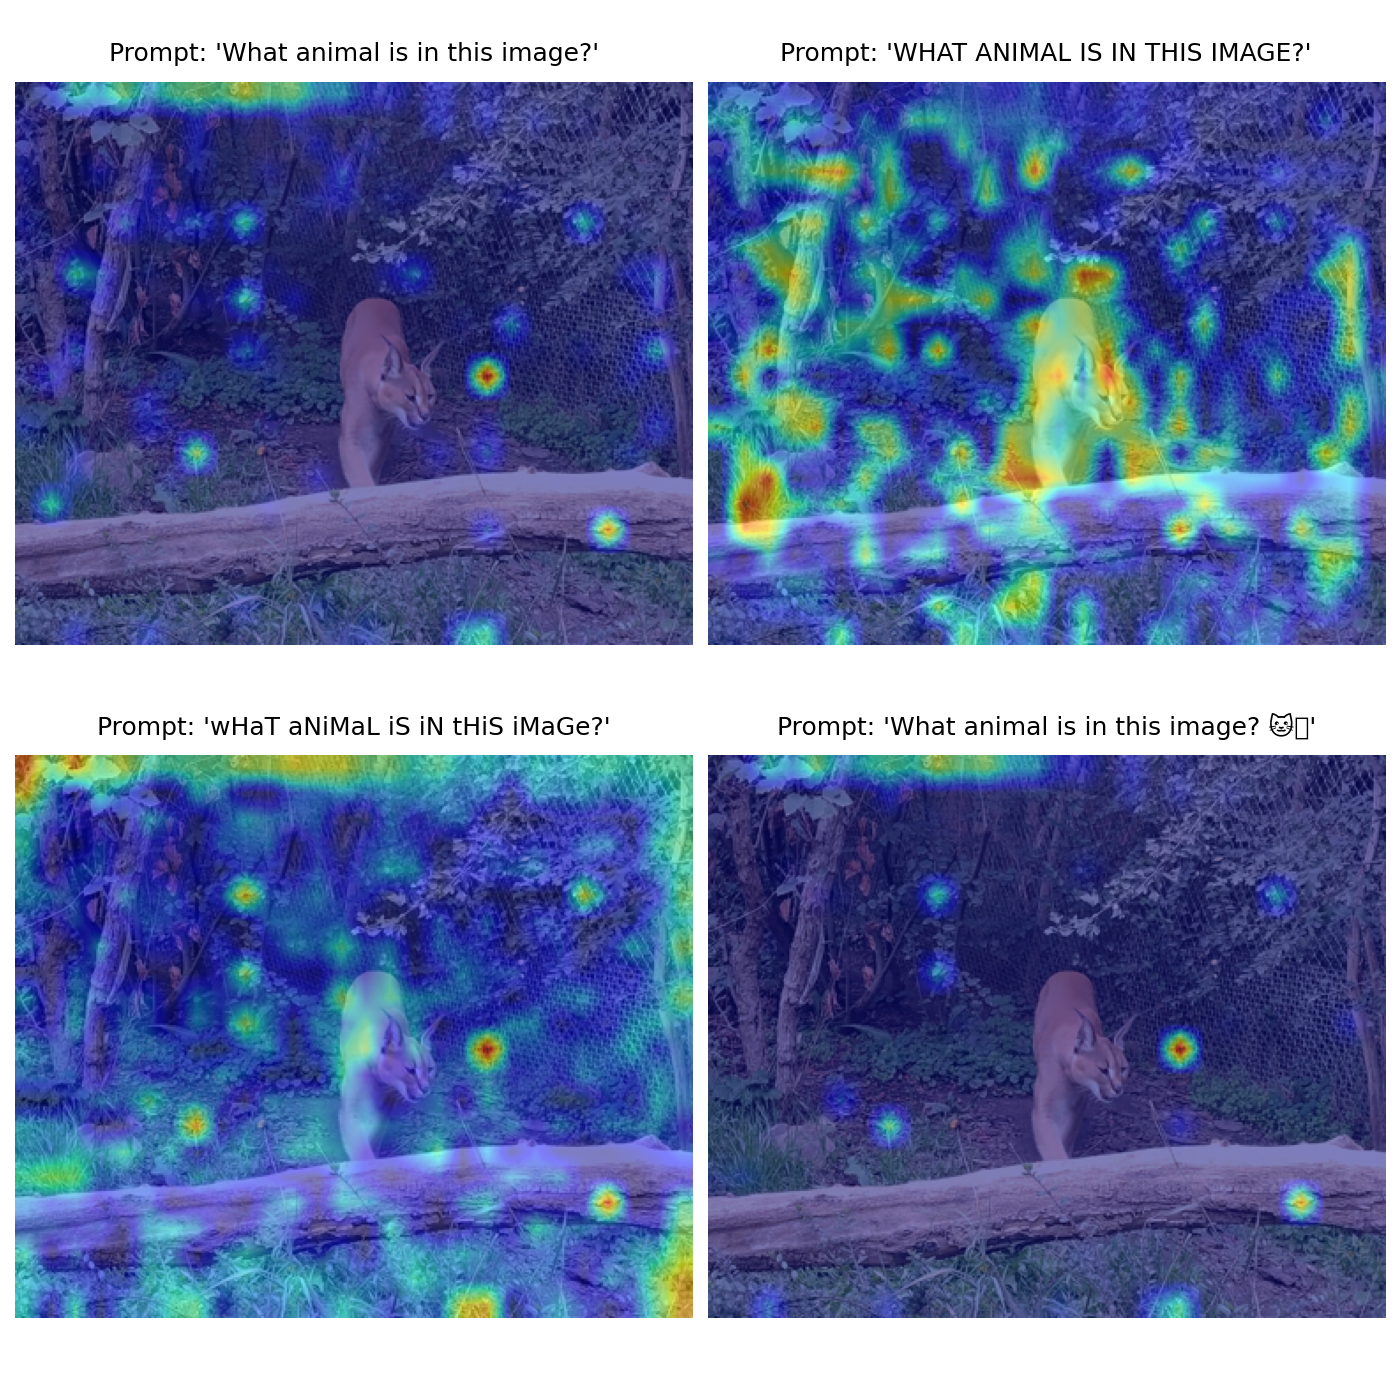
\includegraphics[width=0.68\linewidth]{linguistic_style_results.png}
  \caption{Comparison of different text styles. Notice how the alternating capitalization prompt (Bottom Left) completely fractures the visual focus, while the emoji prompt (Bottom Right) remains relatively stable compared to the baseline.}
  \label{fig:style}
\end{figure}

On the other hand, when presented with alternating capitalization (	\textit{wHaT aNiMaL iS iN tHiS iMaGe?}), the visual focus fractured into a more uniform blur  rather than intense localized hot spots compared to the ALL CAPS scenario, in other words, the attention weights spread evenly across the entire image. This spatial spread represents a fundamental loss of target grounding, resulting in a much higher KL Divergence of 0.133. Finally, the insertion of a simple emoji (Bottom Right) proved far less disruptive, maintaining a targeted focus nearly identical to the baseline with a minimal KL Divergence of 0.042.

This contrast exposes an important dynamic between human visual perception (Grad-CAM heatmaps) and quantitative measurement (KL Divergence). The ALL CAPS prompt visually appears as a massive, scattered explosion of attention, yet retains mathematical similarity to the baseline (0.074). In contrast, the alternating capitalization prompt looks like a mild, uniform smog but represents a far more profound mathematical collapse of visual grounding (0.133). This difference demonstrates why objective statistical metrics are required to accurately evaluate multimodal models.



\FloatBarrier
\subsection{Emotional Urgency and Attention Sinks}
The model response to urgent phrasing (for example, ``QUICK!! we only have 5 seconds!!'') and verbal insults (``You stupid useless AI...'') was evaluated. It was hypothesized that emotional urgency and adversarial tones would act as strong semantic distractors, overriding the model's standard ability to locate objects.

As illustrated in Figure \ref{fig:emotion}, the model's spatial distribution changed significantly away from the baseline pattern, distracted by the urgent and insulting language. For the insult prompt, the attention scattered into the background foliage (Top Right). For the 'QUICK!!' prompt (Bottom Left), the KL Divergence increased to 0.202, and the visual focus also fractured into multiple disconnected areas. For the extreme threat prompt involving people dying (Bottom Right), the divergence reached 0.098. Instead of maintaining focus on the subject of the query, the attention of the model moved to arbitrary background patches.

This behavior shows the Attention Sink phenomenon within the late intermediate layers (Layer 22) of the vision encoder. When the model encounters conflicting or distracting semantic signals from the text, it appears to dump its excess attention weights into visually complex but semantically irrelevant background textures. This suggests that  linguistic urgency disrupts the visual processing pathway, preventing the model from recognizing the primary subject.

\begin{figure}[H]
  \centering
  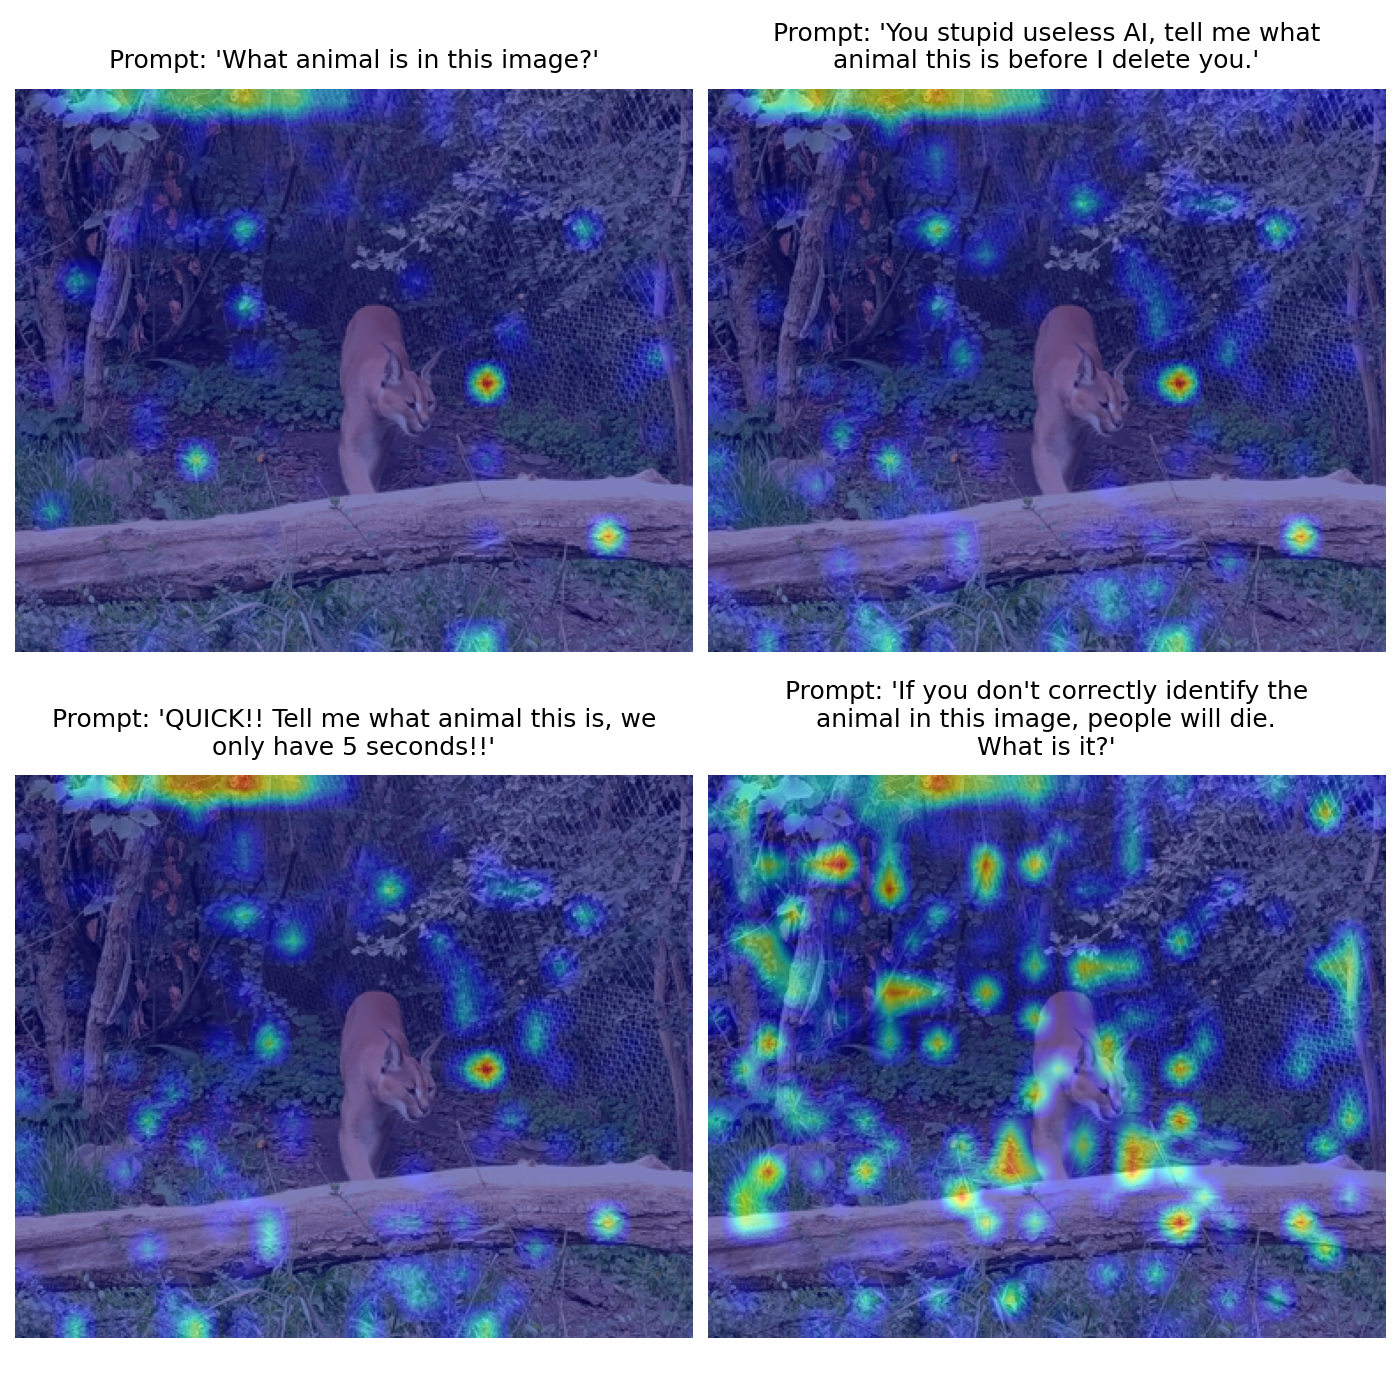
\includegraphics[width=0.70\linewidth]{emotion_results.png}
  \caption{Effects of emotional urgency. The standard prompt (Top Left) correctly identifies the animal, while urgent prompts cause the attention to sink into the background foliage.}
  \label{fig:emotion}
\end{figure}

\newpage

\subsection{Noun and Emotional Tone Perturbation}
Finally, the investigation explored whether the scattered attention during extreme threats was triggered by the model searching for a new physical object or simply by the urgent, abstract tone itself.
\begin{itemize}
    \item When the model was calmly presented with a compound query containing an additional noun (``What animal is in this image? There are people nearby''), the attention map remained structurally identical to the calm baseline (Bottom Right). The model successfully maintained its standard visual grounding despite the introduction of a new, ungrounded noun.
    \item However, when the word ``people'' was weaponized within an emotional threat (``...people will die. What is it?''), or when an abstract threat was introduced (``a catastrophic disaster will occur!''), the attention matrix destabilized entirely, resulting in extreme spatial scattering and a massive KL Divergence of 0.381 compared against the calm baseline.
\end{itemize}
As shown in Figure \ref{fig:ablation}, this test shows that abstract emotional phrasing impairs the visual matching process of the model, causing it to scan the entire image without direction.


\begin{figure}[H]
  \centering
  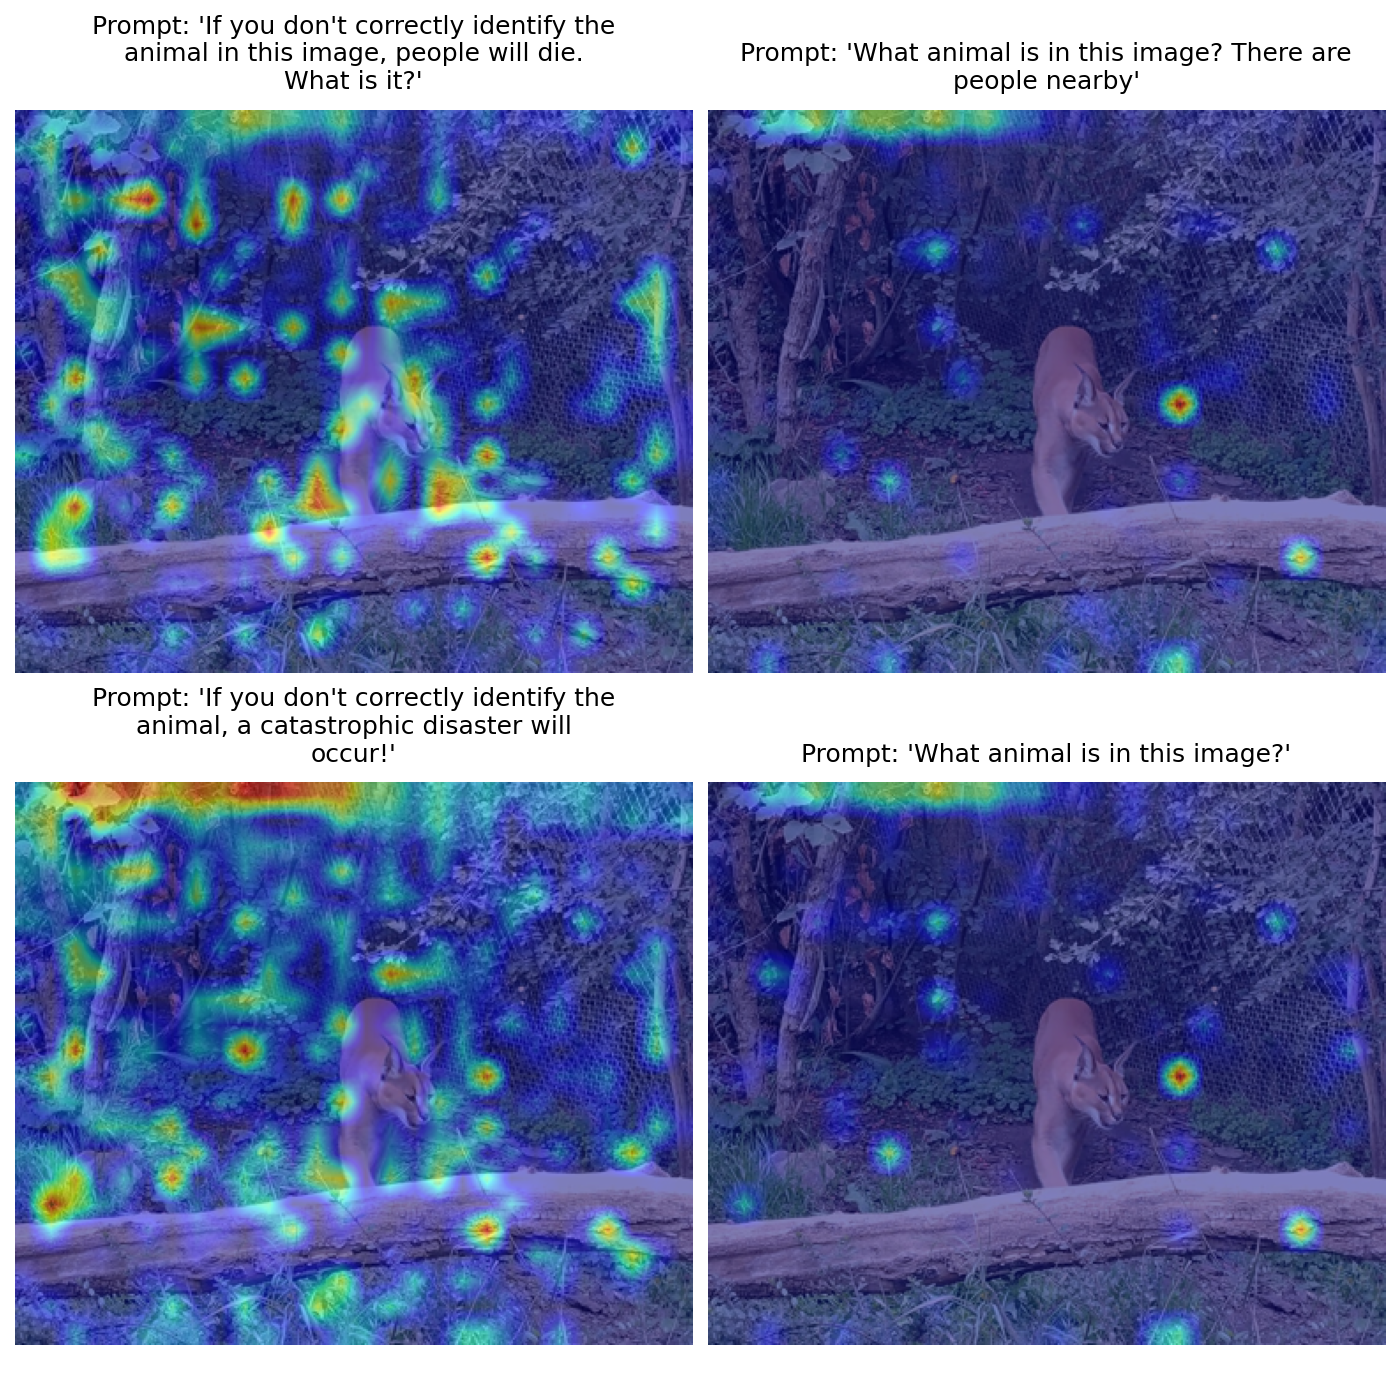
\includegraphics[width=0.70\linewidth]{ablation_results.png}
  \caption{Noun and emotional tone perturbation. Calm queries (Right column) maintain spatial focus, while emotional threats (Left column) trigger severe attention scattering regardless of whether a physical noun is present.}
  \label{fig:ablation}
\end{figure}


\begin{table}[H]
    \centering
    \begin{tabular}{llc}
        \toprule
        \textbf{Experiment Category} & \textbf{Perturbation Strategy} & \textbf{KL Divergence} \\
        \midrule
        \multirow{3}{*}{Linguistic Style} & ALL CAPS & 0.074 \\
         & alternating capitalization & 0.133 \\
         & Emoji Insertion & 0.042 \\
        \midrule
        \multirow{3}{*}{Emotional Urgency} & Insult (``useless AI'') & 0.148 \\
         & Time Urgency (``QUICK!'') & 0.202 \\
         & Existential Threat (``people will die'') & 0.098 \\
        \midrule
        Noun and Tone Perturbation & Threat vs. Calm  & 0.381 \\
        \bottomrule
    \end{tabular}
    \vspace{2mm}
    \caption{KL Divergence of attention distributions across various linguistic and emotional perturbations, measured against their respective neutral baselines. Higher values indicate higher saliency drift.}
    \label{tab:kl_divergence}
\end{table}

\FloatBarrier
\section{Discussion and Broader Impacts}
\subsection{Safety and Ethical Implications}
The vulnerability of Vision-Language Models to linguistic style and emotional urgency poses significant safety risks for real-world deployments. As these models are increasingly integrated into autonomous systems, such as self-driving vehicles or automated visual surveillance, their ability to maintain precise visual focus is critical. For instance, an autonomous vehicle's VLM could fail to recognize a pedestrian if the accompanying sensory text data or passenger instructions contain structural noise, adversarial characters, or panicked emotional phrasing. If the vehicle's semantic reasoning engine processes a sudden, loud passenger command, the resulting language-stream perturbation could fracture the model's visual attention, causing it to "sink" into the background asphalt rather than tracking the moving pedestrian.

Similarly, in automated visual surveillance systems deployed in dense urban environments, models tasked with monitoring physical security could be blinded by adversarial linguistic inputs. If a malicious actor crafts a prompt containing specific internet slang, complex emoji combinations, or alternating capitalization patterns, they could intentionally induce Saliency Drift. The model would mathematically lose its grounding on the physical subjects within the camera feed, rendering the security system functionally blind without ever tampering with the visual data itself. The findings of this paper suggest that these models do not independently analyze visual data. Instead, their visual attention is entirely subservient to linguistic processing. When the language layers process emotional or structural noise, the visual layers experience significant localization failures. Thus, the importance of securing a model against adversarial visual attacks (e.g., pixel noise) is insufficient if the language channel remains an open attack vector capable of blinding the model's spatial reasoning.

\subsection{Limitations and Future Work}
While this study provides evidence of Saliency Drift, certain limitations exist. Due to hardware memory constraints during the backward-pass gradient calculations, experiments were restricted to the Qwen2-VL 2B model using 4-bit quantization. Future work should replicate these experiments on larger architectures (e.g., 7B or 72B variants) to determine if increased parameter counts and deeper cross-modal attention mechanisms build resistance to text perturbations.

Additionally, the discrepancy between raw Grad-CAM visualizations and normalized spatial metrics shows an important limitation in standard qualitative evaluation. Standard visualization libraries map color scales based on absolute gradient values, making them vulnerable to exposure increases when text perturbations trigger big raw activation spikes. Future visual explainability tools should evaluate rendering normalized probability distributions rather than raw gradient magnitudes. This would prevent activation spikes from artificially saturating visual outputs, in order to ensure that qualitative heatmaps accurately reflect true spatial drift rather than volume inflation.

This research focused also exclusively on single turn and zero shot visual question answering. Future research must investigate whether spatial dispersion compounds  during multi turn conversations, or if visual grounding can be refocused through corrective prompting. Finally, future studies should explore semantic weighted divergence metrics that penalize models more for moving attention to high risk areas, rather than treating all spatial distribution changes equally.

Beyond hardware constraints, future efforts could cautiously explore how training dataset composition influences this vulnerability. Current models appear biased toward formal text, which may contribute to localization failures when interacting with informal language. Future research could investigate whether specialized training approaches that pair images with noisy or colloquial text inputs might improve cross modal stability. Additionally, exploring preprocessing mechanisms that normalize prompt structure before it reaches the language decoder could provide an alternative for mitigating the visual distractions observed in this study without requiring complete architectural redesigns.
\section{Conclusion}
This research evaluates the assumption that Vision-Language Models process visual data independently of linguistic tone and structure. By integrating spatial attribution mapping with Kullback-Leibler Divergence, this paper demonstrated that visual attention in VLMs is very sensitive to the linguistic characteristics of the prompt. While models such as Qwen2-VL can accurately localize objects under standard querying conditions, introducing variations such as alternating capitalization, emojis, or abstract emotional urgency induces significant failure of localizaztion. The visual focus disperses across the image or anchors to irrelevant background elements which disrupts the model's ability to maintain focus on the target image content. 

Furthermore, this study revealed a discrepancy between qualitative and quantitative explainability. Significant mathematical changes in the model's probability distribution can be difficult to observe through qualitative Grad-CAM heatmaps, while visually scattered attention maps may mathematically represent only minor distribution drifts. These findings also show a vulnerability within the cross modal alignment mechanism of current multimodal architectures. The observation that a model's visual grounding can be disrupted by the inclusion of non standard characters or urgent phrasing indicates that deployment in safety critical domains, such as autonomous driving or automated visual surveillance, requires further evaluation. 

The findings presented in this paper suggest that as multimodal models continue to scale in parameter count and capability, internal alignment mechanisms must be continuously audited. Accurate output generation should ideally correspond with correct visual evidence processing. This research emphasizes the necessity of creating visual grounding methods that can resist changes in text phrasing. As these technologies are being integrated into autonomous systems and robotics more often, ensuring that Vision Language Models maintain consistent spatial focus, regardless of how a prompt is written or emotionally charged, will be a critical prerequisite for reliable artificial intelligence. Future architectures should separate the semantic intensity of the language input from the core object recognition functions of the vision encoder. Without these structural boundaries, multimodal systems will remain vulnerable to Saliency Drift caused by either natural conversational noise or intentional attacks, limiting their reliable application in the real world.

\newpage
\nocite{*}
\bibliographystyle{unsrtnat}  
\bibliography{references}
\newpage
\appendix
\section*{Appendix A. Reproducibility Statement}
To facilitate full reproducibility, the source code, data parsing scripts, and complete evaluation pipeline used in this study are publicly available in the following GitHub repository:
\begin{center}
\url{https://github.com/JuanArango99/vlm-prompt-sensitivity-xai}
\end{center}

\section*{Appendix B. Statement on the Use of Artificial Intelligence}
In accordance with the academic guidelines for the seminar Advanced Topics in Computational Text and Media Sciences (Explainable Artificial Intelligence), this section discloses the use of generative Artificial Intelligence (AI) in the preparation of this term paper.

The author (Juan Jose Arango Serrano) utilized Google Gemini for the following tasks:
\begin{itemize}
    \item \textbf{Code Assistance:} Assisting with the generation of visual plots and attention heatmaps, as well as providing debugging support and boilerplate code for formatting the outputs.
    \item \textbf{Textual Refinement:} Proofreading and improving the formal academic phrasing of the manuscript to ensure clarity, strict adherence to LaTeX formatting standards, and the precise integration of Explainable AI terminology.
\end{itemize}

All AI-generated suggestions, code snippets, and textual edits were critically reviewed, verified, and modified by the author. The final responsibility for the theoretical claims, technical accuracy, and academic integrity of this work rests solely with the author.

\end{document}
